
%(BEGIN_QUESTION)
% Copyright 2009, Tony R. Kuphaldt, released under the Creative Commons Attribution License (v 1.0)
% This means you may do almost anything with this work of mine, so long as you give me proper credit

Undersøk de ulike konfigurasjonsfeltene for en guidet bølgeradartransmitter vist i dette skjermbildet (fra PC med Emerson AMS-programvare, koblet mot en Rosemount model 3300 nivåtransmitter), og forklar betydningen av hvert felt:

$$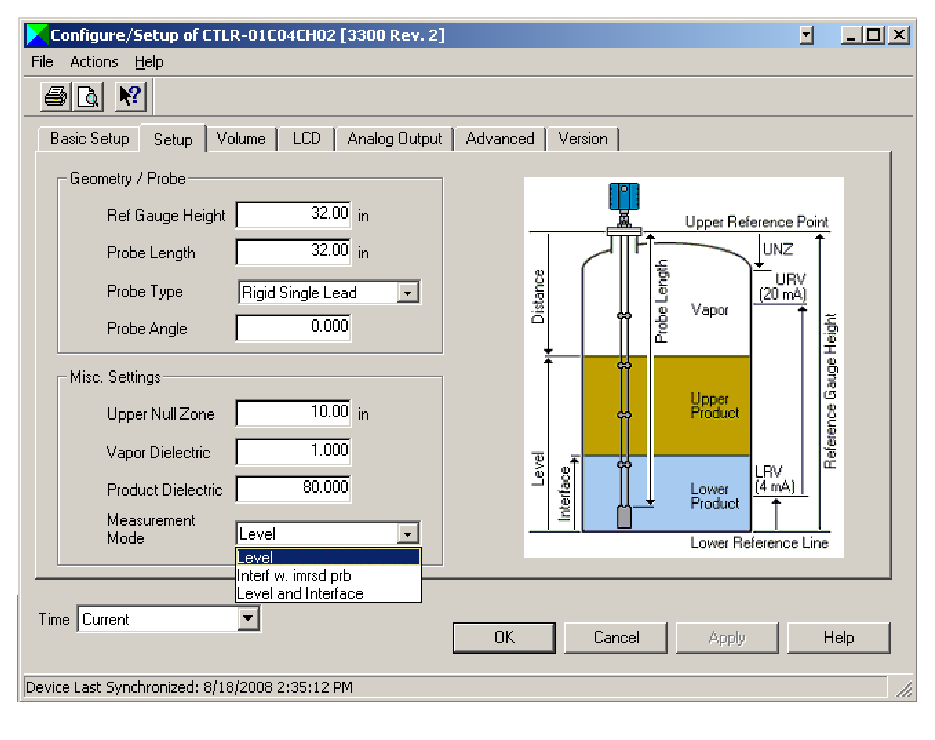
\includegraphics[width=15.5cm]{i00292x01.eps}$$

\vskip 20pt \vbox{\hrule \hbox{\strut \vrule{} {\bf Forslag til sokratisk diskusjon} \vrule} \hrule}

\begin{itemize}
\item{} Mener du det er realistisk å sette spenn for en GWR-transmitter lik probelengden?  Hvorfor/hvorfor ikke?
\item{} Hva betyr valget ``Interf w. imrsd prb'', spesielt sammenlignet med de andre målemodusvalgene?
\item{} Hvilken betydning har innstillingen ``Probe Angle''?
\end{itemize}

\underbar{file i00292}
%(END_QUESTION)





%(BEGIN_ANSWER)

%(END_ANSWER)





%(BEGIN_NOTES)

%INDEX% Measurement, level: radar

%(END_NOTES)
